
\section{Optimizing the Ramp scenario}
\label{ramp_optimization}

Figure~\ref{summary_currentramp} shows the full endcap results showing the coolant temperature,
BPOL12V load current (from ABCs and HCCs), sensor leakage current, and sensor power headroom factor
for two scenarios. On the left is the $-35$~$^{\circ}$C cooling scenario, and on the right is the
currently proposed ramp scenario. As a reminder, the $-35$~$^{\circ}$C scenario is problematic because
the BPOL12V load current exceeds the specification of 4A in R1. On the other hand, the ramp scenario
produces spikes in sensor leakage current throughout the 14-year detector lifetime.

We can optimize the coolant temperature ramp to maintain the BPOL12V load current below a 4A threshold
and reduce leakage sensor current spikes. To guide the study, the model is run for constant cooling
scenarios at 5$^{\circ}$C
intervals, using the Endcap R1 module (the module with the highest BPOL12V load current). 
The results are shown in Figure~\ref{dedicated_study}. The black
dotted lines indicate different ramping scenarios. The model assumes that changing temperature from
year-to-year is equivalent to jumping between the constant cooling scenarios. This is a consequence of
the current modeling of the TID bump and sensor leakage in the model.

The plots on the right in Figure~\ref{dedicated_study} represent a scenario that selects the coldest
coolant temperature that maintains the BPOL12V current load below 4A. This scenario introduces only
one additional peak in the sensor leakage current (at year 2), and the current at this peak is kept
below 0.5~mA. That cooling scenario is:
\begin{equation}
T = {-}25~|~{-}25~|~{-}35~|~{-}35~|~{-}35~|~{-}35~|~{-}35~|~{-}35~|~{-}35~|~{-}35~|~{-}35~|~{-}35~|~{-}35~|~{-}35
\label{eq:proposal1}
\end{equation}

\begin{figure}[ht!]
\begin{subfigure}[t]{0.50\textwidth}
\begin{center}
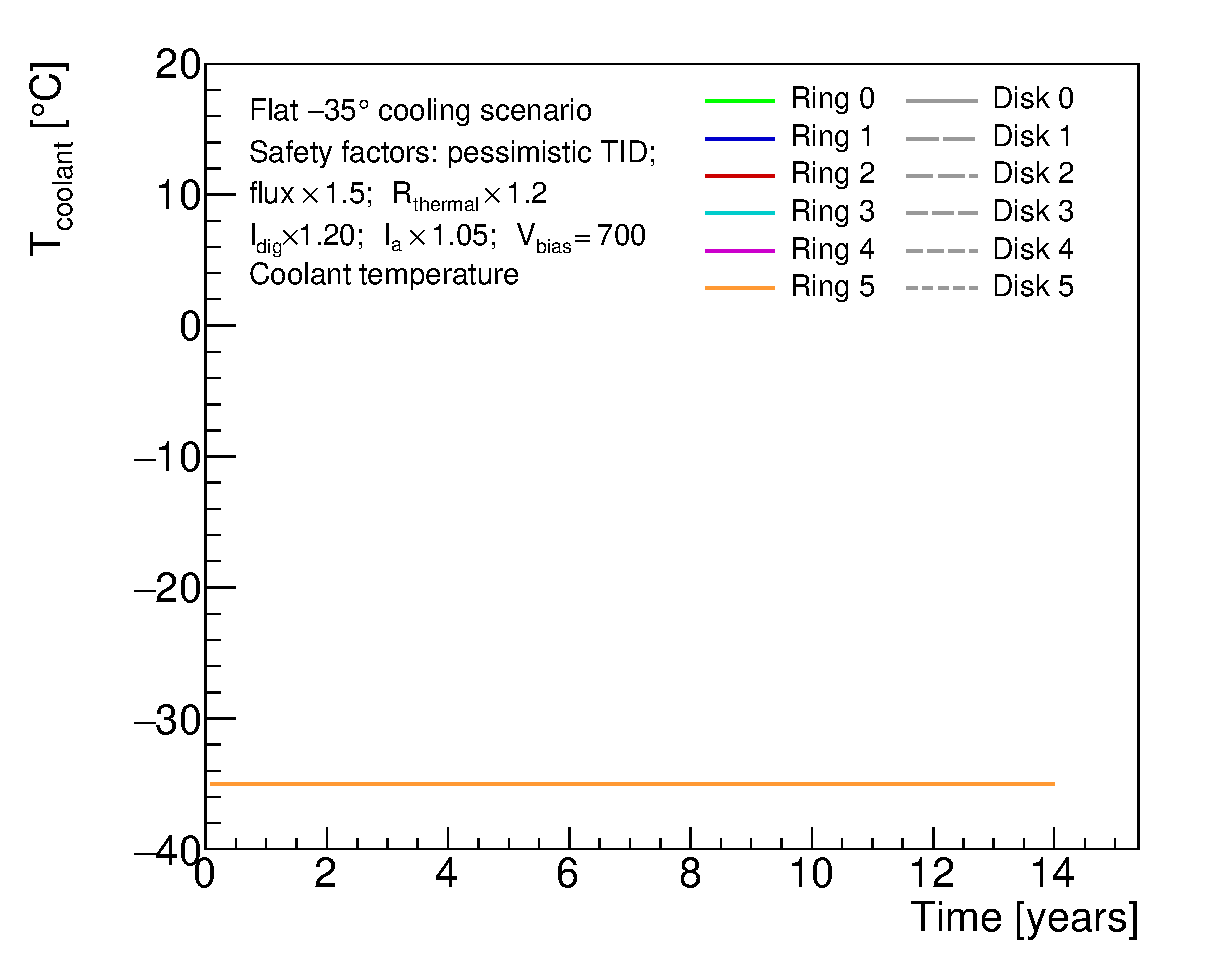
\includegraphics[width=0.74\linewidth]{figures/studies/Endcap_CoolantTemperature_WorstCase.eps}
\includegraphics[width=0.74\linewidth]{figures/studies/Endcap_FeastCurrent_WorstCase.eps}
\includegraphics[width=0.74\linewidth]{figures/studies/Endcap_SensorCurrent_WorstCase.eps}
\includegraphics[width=0.74\linewidth]{figures/studies/Endcap_SensorQHeadroom_WorstCase.eps}
\end{center}
\caption{Flat $-35^{\circ}~C$ scenario}
\end{subfigure}
\begin{subfigure}[t]{0.50\textwidth}
\begin{center}
\includegraphics[width=0.74\linewidth]{figures/studies/Endcap_CoolantTemperature_Ramp_m35.eps}
\includegraphics[width=0.74\linewidth]{figures/studies/Endcap_FeastCurrent_Ramp_m35.eps}
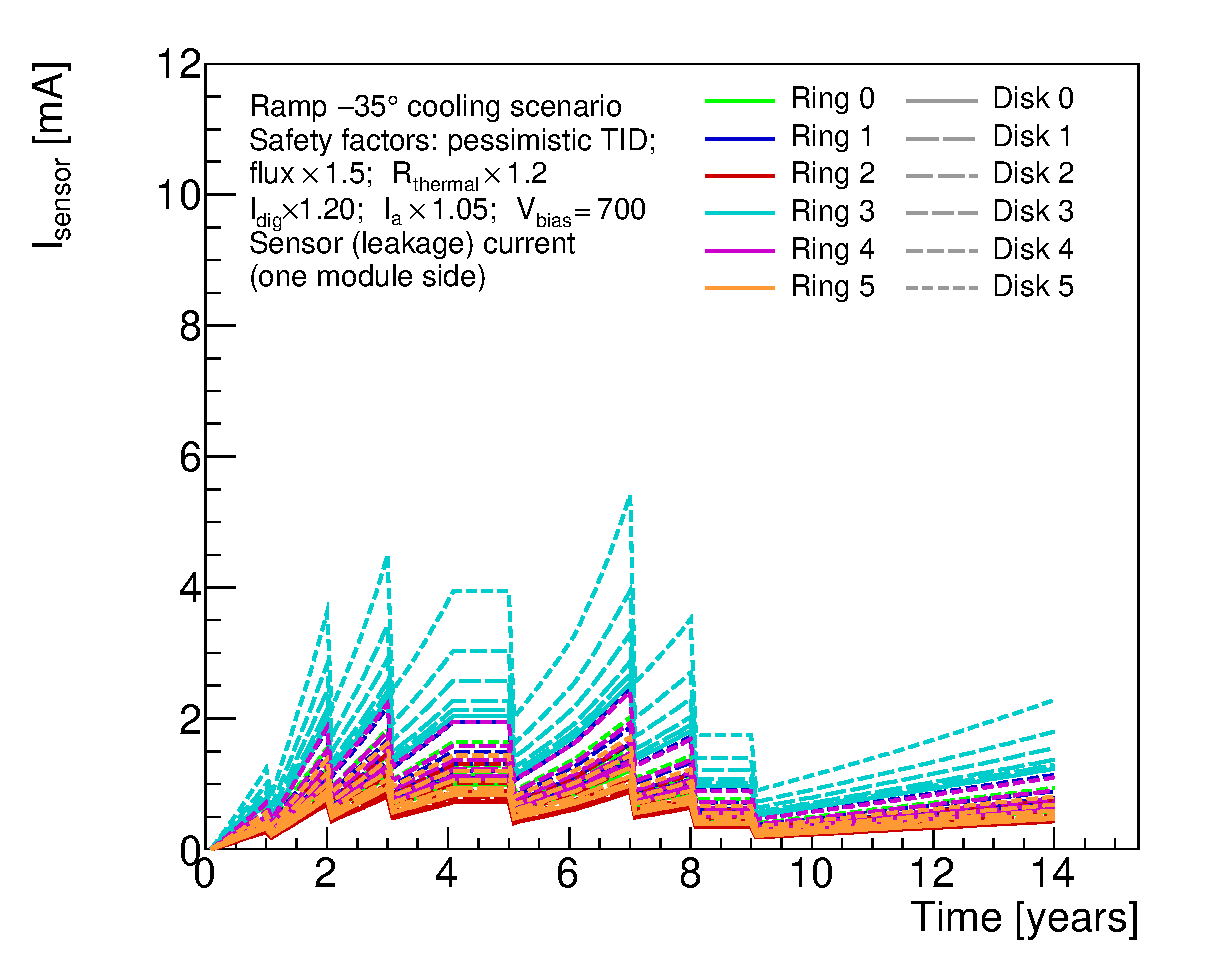
\includegraphics[width=0.74\linewidth]{figures/studies/Endcap_SensorCurrent_Ramp_m35.eps}
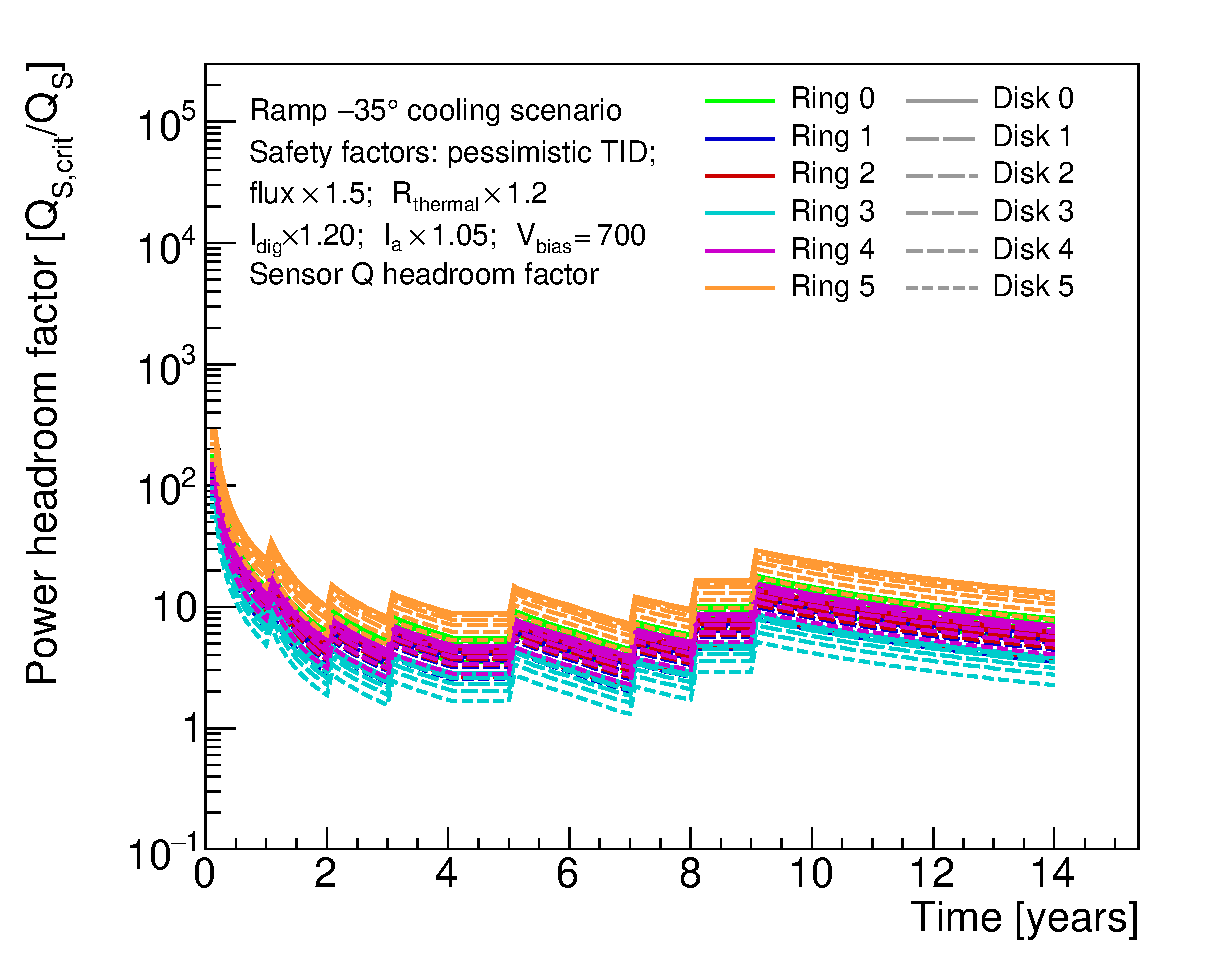
\includegraphics[width=0.74\linewidth]{figures/studies/Endcap_SensorQHeadroom_Ramp_m35.eps}
\end{center}
\caption{Ramp scenario proposed by Georg}
\end{subfigure}
\caption{BPOL12V current load with all safety factors applied. Left: $-35$~$^{\circ}$C coolant
temperature. Right: the canonical ``Ramp'' scenario. Pictured is the coolant temperature
(as a sanity check), BPOL12V current load (from ABCs and HCCs), sensor leakage current, and sensor Q
headroom factor.}
\label{summary_currentramp}
\end{figure}

\begin{figure}[ht!]
\begin{subfigure}[t]{0.50\textwidth}
\begin{center}
\includegraphics[width=0.74\linewidth]{figures/studies/CoolantTemperature_CompareR1_Ramp.eps}
\includegraphics[width=0.74\linewidth]{figures/studies/FeastCurrent_CompareR1_Ramp.eps}
\includegraphics[width=0.74\linewidth]{figures/studies/SensorCurrent_CompareR1_Ramp.eps}
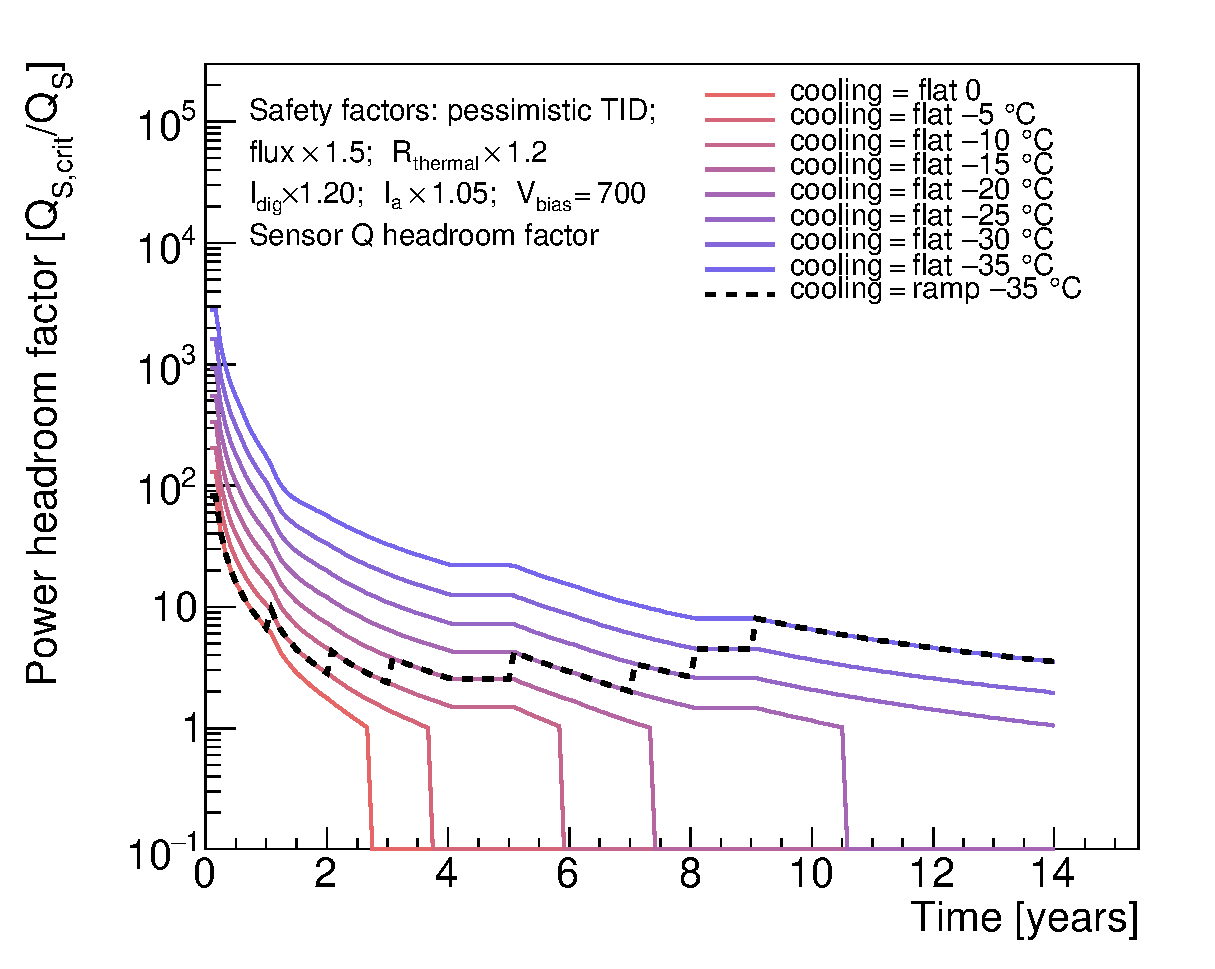
\includegraphics[width=0.74\linewidth]{figures/studies/SensorQHeadroom_CompareR1_Ramp.eps}
\end{center}
\end{subfigure}
\begin{subfigure}[t]{0.50\textwidth}
\begin{center}
\includegraphics[width=0.74\linewidth]{figures/studies/CoolantTemperature_CompareR1_Proposal.eps}
\includegraphics[width=0.74\linewidth]{figures/studies/FeastCurrent_CompareR1_Proposal.eps}
\includegraphics[width=0.74\linewidth]{figures/studies/SensorCurrent_CompareR1_Proposal.eps}
\includegraphics[width=0.74\linewidth]{figures/studies/SensorQHeadroom_CompareR1_Proposal.eps}
\end{center}
\end{subfigure}
\caption{The performance of the R1 module in different cooling scenarios, with all safety factors on.
The model is run for flat cooling scenarios at 5$^{\circ}$C intervals. On the left, the ramp scenario
is shown as a dotted black line. On the right, a different optimized scenario is shown.
 }
\label{dedicated_study}
\end{figure}

%% Figure~\ref{new_proposal} applies this scenario (``Two years at  $-35$~$^{\circ}$C'') to the other
%% endcap modules. The behavior seems acceptable for all endcap modules. This type of study can be
%% repeated to optimize other desired qualitites in a ramping scenario.

%% \begin{figure}[ht!]
%% \begin{center}
%% \includegraphics[width=0.49\linewidth]{figures/studies/Endcap_CoolantTemperature_Proposal.eps}
%% \includegraphics[width=0.49\linewidth]{figures/studies/Endcap_FeastCurrent_Proposal.eps}
%% \includegraphics[width=0.49\linewidth]{figures/studies/Endcap_SensorCurrent_Proposal.eps}
%% \includegraphics[width=0.49\linewidth]{figures/studies/Endcap_SensorQHeadroom_Proposal.eps}
%% \end{center}
%% \caption{Proposal scenario: two years of running at $-25^{\circ}~C$, followed by running at
%% $-35^{\circ}~C$. The plots show the performance on all endcap modules.
%% }
%% \label{new_proposal}
%% \end{figure}

\clearpage

\subsection{Ramp proposal: Highest coolant temperature while keeping sensor current maximum at
end-of-life}

When deciding on the ramp scenario, there can be a balance between keeping a safe BPOL12V current
and avoiding large sensor currents intermittently before end-of-life. In the following, the coolant
temperature at end-of-life is set at $-35^\circ$~C, and the coolant ramp is selected such that
the sensor leakage current in a given year is always below the end-of-life sensor current.
Because the endcap R3 has the highest leakage current, it is used as the benchmark for this study.
The ramp that fulfils this criteria in R3 is:
\begin{equation}
T = 0~|~{-}10~|~{-}20~|~{-}20~|~{-}20~|~{-}25~|~{-}30~|~{-}30~|~{-}30~|~{-}35~|~{-}35~|~{-}35~|~{-}35~|~{-}35
\label{eq:proposal2}
\end{equation}

Figure~\ref{new_proposal2_r3} shows the R3 behavior in this case. The top-right plot (sensor leakage
current) is the one used to visually guide the coolant temperature selection.

\begin{figure}[ht!]
\begin{center}
\includegraphics[width=0.37\linewidth]{figures/studies/CoolantTemperature_CompareR3_Proposal2.eps}
\includegraphics[width=0.37\linewidth]{figures/studies/SensorCurrent_CompareR3_Proposal2.eps}\\
\includegraphics[width=0.37\linewidth]{figures/studies/FeastCurrent_CompareR3_Proposal2.eps}
\includegraphics[width=0.37\linewidth]{figures/studies/SensorQHeadroom_CompareR3_Proposal2.eps}
\end{center}
\caption{R3 performance using the cooling ramp scenario from Eq.~\ref{eq:proposal2}.
}
\label{new_proposal2_r3}
\end{figure}

Figure~\ref{new_proposal2} shows the performance of this new ramp scenario on the rest of the endcap
modules. The full endcap results are also calculated in the main tables in Section~\ref{results}.
Compared to the current ramp, the new scenario has +2.5\% more LV power but 1/2 as much HV power and
58\% less sensor current (from 5.42~mA $\rightarrow$ 2.28~mA in R3).

\begin{figure}[ht!]
\begin{center}
\includegraphics[width=0.49\linewidth]{figures/studies/Endcap_CoolantTemperature_Proposal2.eps}
\includegraphics[width=0.49\linewidth]{figures/studies/Endcap_FeastCurrent_Proposal2.eps}
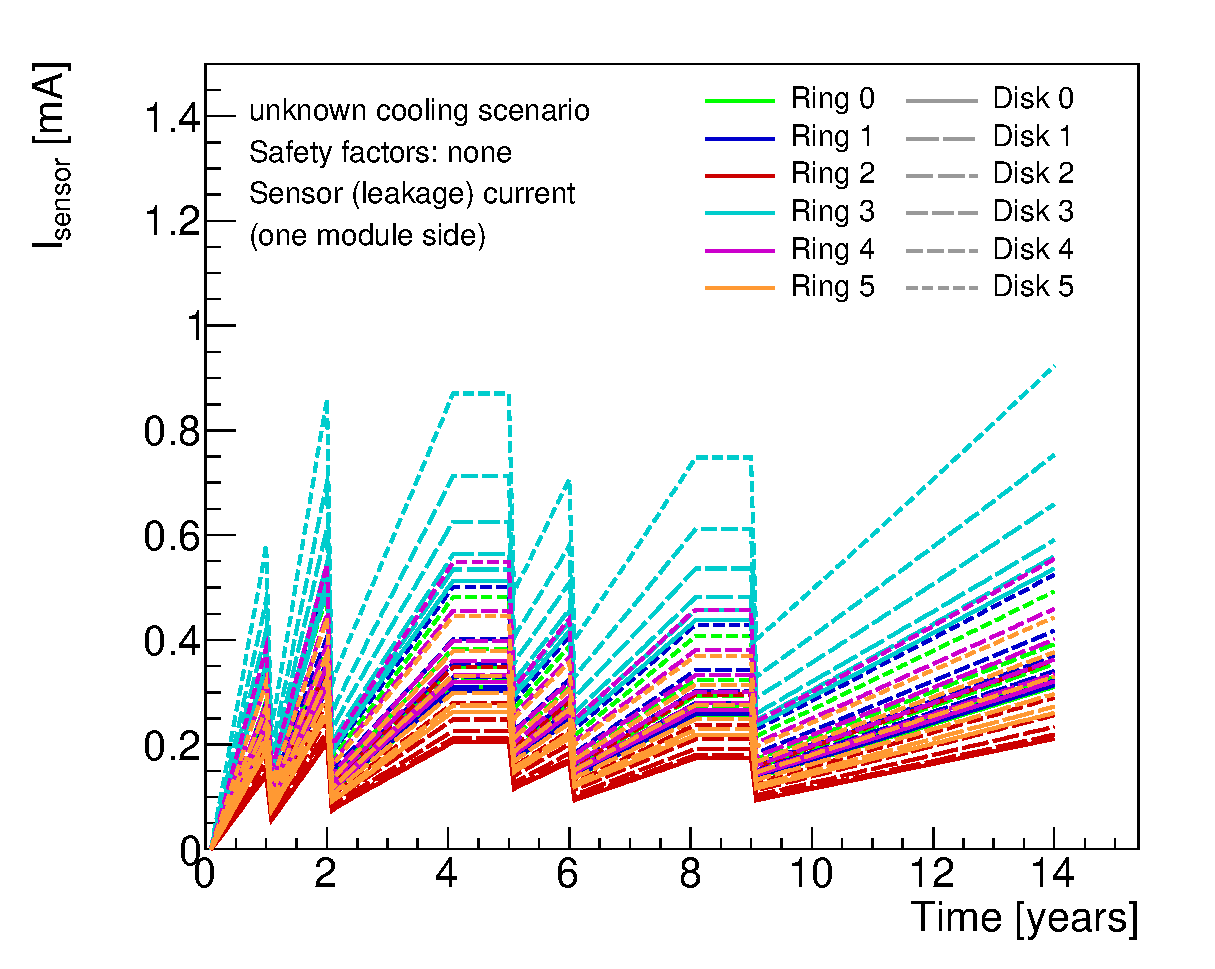
\includegraphics[width=0.49\linewidth]{figures/studies/Endcap_SensorCurrent_Proposal2.eps}
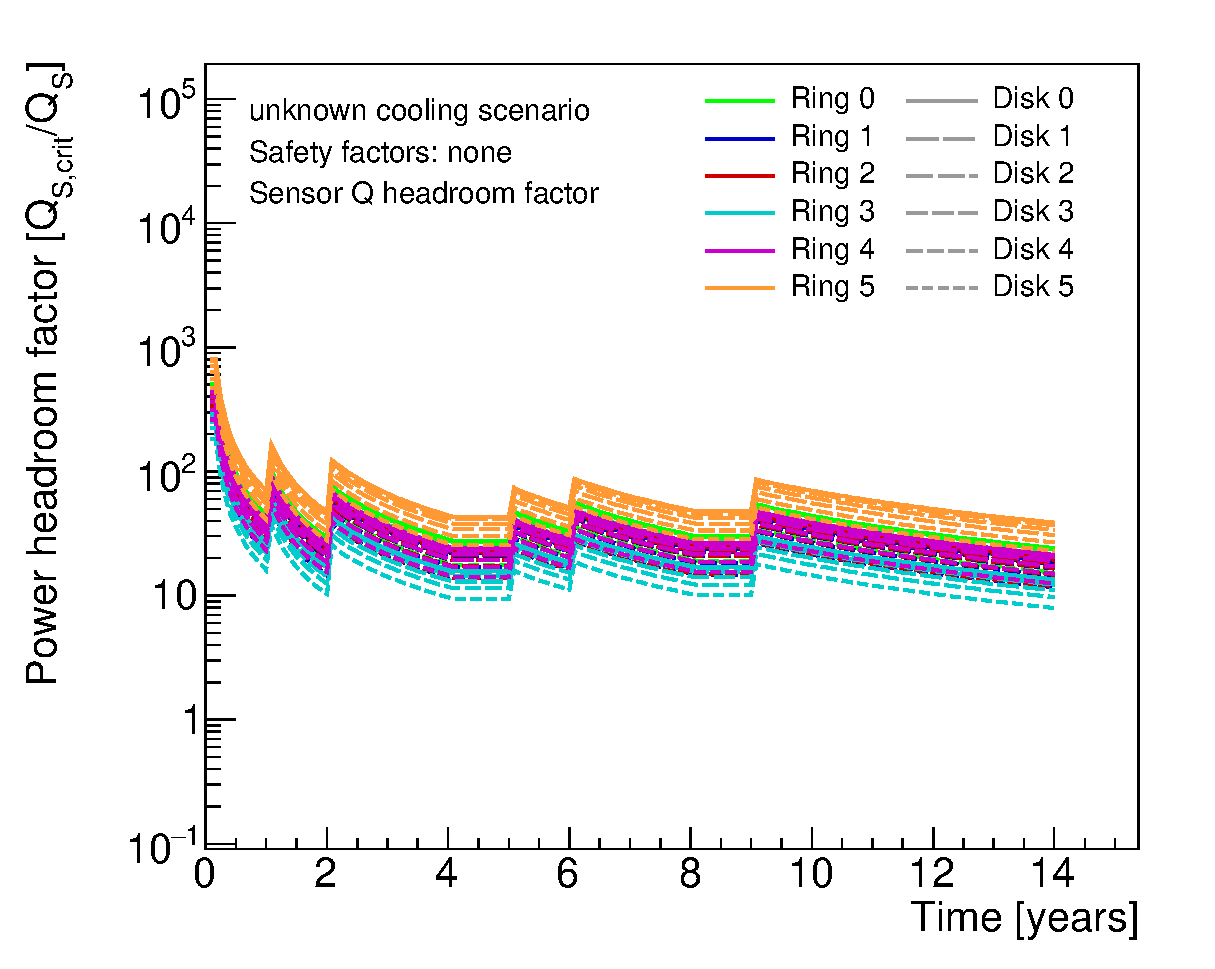
\includegraphics[width=0.49\linewidth]{figures/studies/Endcap_SensorQHeadroom_Proposal2.eps}
\end{center}
\caption{ The effect of cooling ramp scenario from Eq.~\ref{eq:proposal2} on the barrel modules.
}
\label{new_proposal2}
\end{figure}

\subsection{Summary of studies}

The studies above illustrate that a range of ramping scenarios are viable. The ramping scenario of
Eq.~\ref{eq:proposal1} is the coldest ramp available that keeps the R1 BPOL12V below 4A. The ramping
scenario of Eq.~\ref{eq:proposal2} is the warmest available ramp that avoids a maximum sensor leakage
current before the end-of-life. Any ramping scenario that falls in between will also meet these two
conditions.
